\subsection{SMT}

\begin{enumerate}
	\item BR
	\item BR
\end{enumerate}

\begin{figure}[htb]
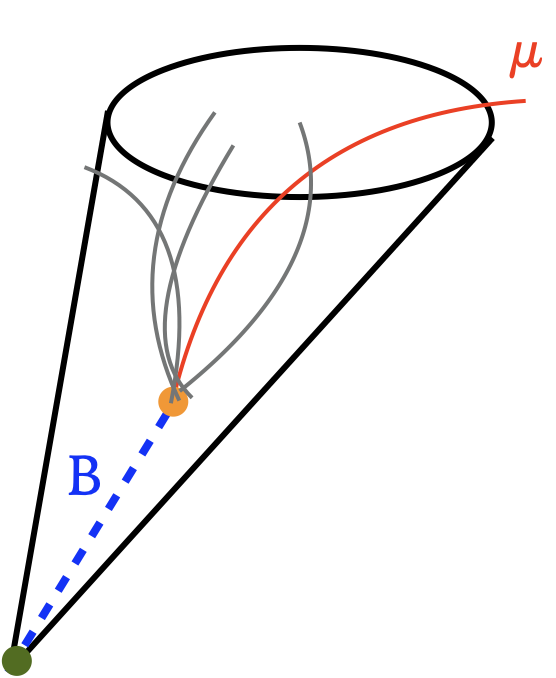
\includegraphics[width=.3\textwidth]{figures/ftag/SMT-image}
\caption{Illustration of a semileptonic $B$-decay}
\end{figure}

\begin{table}[h!]
  \centering
    \begin{tabular}{l | l } % <-- Alignments: 1st column left, 2nd middle and 3rd right, with vertical lines in between
      \textbf{Input} & \textbf{Description}  \\
      \hline
      \hline
  	$s_{d0}$ & $d_0 / \sigma_{d0}$: Transverse IP significance \\
	$s_{z0}$ & $z_0 \sin \theta / \sigma_{z0 \sin \theta}$: Longitudinal IP significance \\
%	$\log \pT^{frac}$ & $\log \pT^{track} / \pT^{jet}$: Logarithm of fraction of the jet $\pT$ carried by the track \\
%	$\log \Delta R$ & Logarithm of opening angle between the track and the jet axis \\    \end{tabular}
    \caption{Track features used as inputs for RNNIP and DIPS algorithms.}
    \label{table:inputs}
\end{table}

\textbf{I think Rafael added new variables too:}